\documentclass[a4paper,10pt,fleqn]{article}
\usepackage{mathtext}
\usepackage[T2A]{fontenc}
\usepackage[utf8x]{inputenc}
\usepackage[english,ukrainian]{babel}
\usepackage{amsfonts,amsmath,stmaryrd}
\usepackage{indentfirst}
\usepackage[pdftex]{color,graphicx}
\usepackage{float}
\usepackage{subfig}
\usepackage[protrusion=true,expansion=true]{microtype}
%\usepackage{iwona}
%\usepackage{cmbright}
%\usepackage[math]{anttor}
%\usepackage[condensed,math]{anttor}
%\usepackage[math]{kurier}
\usepackage{literat}

\DeclareGraphicsRule{.jpeg}{.bmp}{}{}
\textwidth 16 cm
\textheight 24.5cm
\topmargin -1 cm
\evensidemargin 0 cm
\oddsidemargin 0 cm
\normalfont
\title{Індуктивні методи моделювання навігації агента}
\author{Накрийко Андрій}

\begin{document}
\selectlanguage{ukrainian}
\maketitle

\begin{abstract}
This article describes two approaches to solving an agent navigation task. Starting with the neural network-based controller taught on set of expert rules small practical use due to a lack of state-space complexity scalability is concluded. With an inductive approach called reinforcement learning in which mobile agent learns just from interaction with environment one can get controller more suited to real-world tasks. That is proven by a good agent performance in robot navigation problem. Detailed discussion of different algorithm parameters and their impact on performance, speed and stability of the learning process is provided.
\end{abstract}


\section{Вступ}

Робототехніка за останні десятиліття пройшла довгий шлях у своєму розвитку і з кожним роком набирає все більших обертів. І хоч до успішного розв'язання основних проблем робототехніки ще далеко, роботи знаходять застосування у все ширшому колі задач. Одним з важливих і дуже цікавих розділів робототехніки є мобільні роботи. Вони ставлять перед дослідниками чимало складних та досі недостатньо добре розв'язаних проблем. Однією з таких проблем є задача навігації автономного мобільного агента (робота). 

Ця задача може ставитися у різних формах, але найбільш загальною і складною є задача автономної навігації агента в умовах зовнішнього середовища, про яке наперед немає жодних даних. Тобто агенту не надається інформація про розташування різноманітних перешкод (рухомих та нерухомих) в навколишньому середовищі. Агентом в даному випадку виступає мобільний робот, який здатний рухатися самостійно. Ця задача є предметом досліджень багатьох галузей науки: теорії керування, теорії прийняття рішень, робототехніки, штучного інтелекту, машинного навчання тощо. За останні 20 років людство зробило суттєві кроки вперед у її вирішенні, проте повністю вирішеною проблему вважати ще зарано.

В даній роботі ми розглянули два різних підходи до розв'язання цієї задачі і спробували оцінити переваги та недоліки кожного з них: підхід на основі експертних правил та підхід на основі навчання з підсиленням.


\section{Перший підхід --- експертні правила}

\subsection{Постановка задачі}

Для першого підходу в якості агента був обраний автомобіль з досить реалістичною фізикою руху, завданням якого був неперервний рух без конкретної кінцевої мети. Єдиною вимогою, що ставилася перед агентом, була вимога мінімізувати зіткнення з перешкодами, заздалегідь оминаючи їх. Щоб якомога краще наблизити умови, в яких перебуває віртуальний автомобіль, до реальності, система керування сприймає лише об'єкти, що потрапляють у поле зору, обмежене певним кутом та дальністю огляду. 

Агенту надається інформація у відносних одиницях про те, наскільки близько знаходиться перешкода в межах кожного з трьох секторів ``поля зору'' (рис.~\ref{fig:visible-area}). Керування автомобілем полягає у виборі значення прискорення з обмеженого діапазону та кута повороту керма, також в заданих рамках. Усі вказані величини є дійсними числами.

\begin{figure}
  \centering
  \subfloat[Поле зору автомобіля]{
  	\label{fig:visible-area}
  	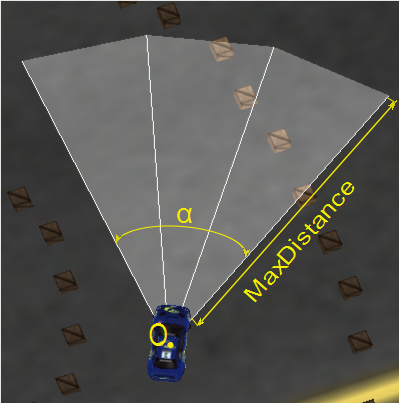
\includegraphics[width=0.38\textwidth]{visible-area}
  }\,
  \subfloat[Автомобіль зупинився і не може здійснити розворот]{
  	\label{fig:car-stuck}
  	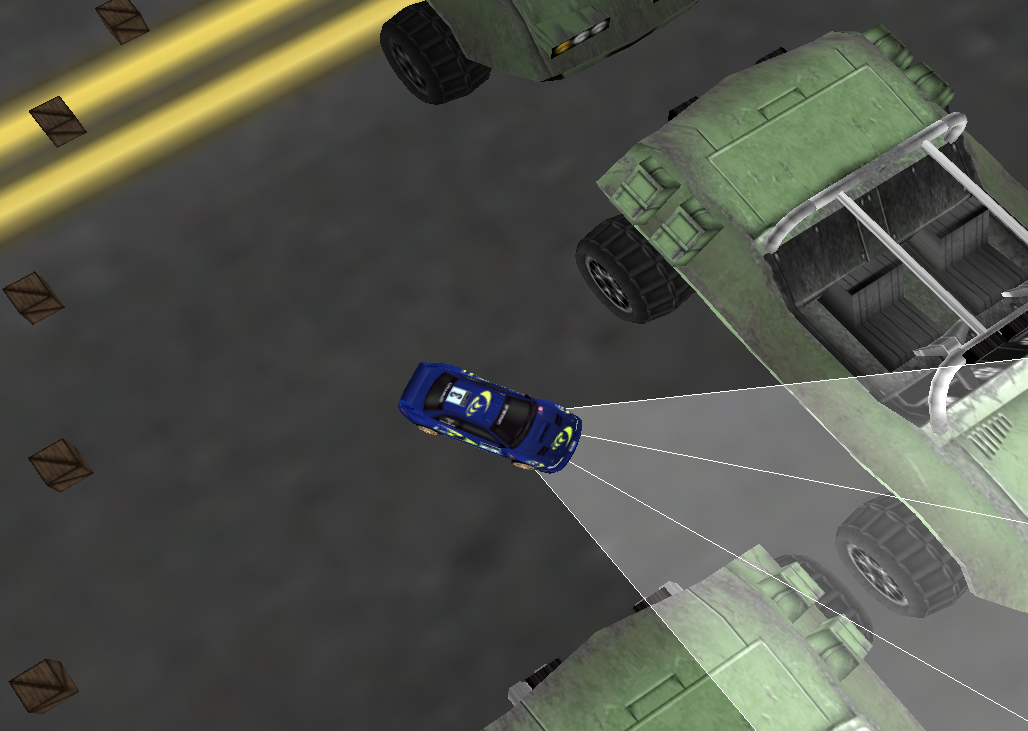
\includegraphics[width=0.54\textwidth]{car-stuck}
  }
  \caption{Ілюстрації до першого підходу}
  \label{fig:car-related}
\end{figure}

\subsection{Експертні правила та штучна нейронна мережа}

Першим підходом до розв'язання задачі керування агентом було використання наперед заданого набору експертних правил, що представляли собою пари еталонних вхідних та бажаних вихідних даних. Вхідними даними був вектор з відстаней до перешкод в трьох секторах поля зору, вихідними даними --- вектор з еталонними прискоренням та кутом повороту. Оскільки усі можливі ситуації описати неможливо, була створена невелика вибірка з близько двадцяти еталонних навчальних пар, а для того, щоб узагальнити ці правила на усі можливі ситуації була використана нейромережа з прямим поширенням сигналу, яка завдяки здатності узагальнювати дані виконувала роль функції керування. Навчання відбувалося популярним алгоритмом зворотнього поширення похибки. Завдяки узагальнюючій властивості нейромережі, ми надіялися отримати контролер, здатний приймати ``осмислені'' рішення в ситуаціях, безпосередньо не заданих в системі правил, шляхом інтерполяції або екстраполяції ``схожих'' правил з навчальної вибірки.

Для перевірки ефективності рішення на основі експертних правил, було створено віртуальне середовище, в якому рухався автомобіль. Керування здійснювалося не через певні дискретні проміжки часу, а в неперервному режимі, як тільки ресурси комп'ютера дозволяли це зробити. Така особливість вносить певну залежність поведінки агента від потужності комп'ютера, на якому виконується симуляція, оскільки більш потужний комп'ютер дає можливість більш оперативного керування подальшим рухом агента. 

\subsection{Результати підходу на основі експертних правил}

Результати не можна охарактеризувати однозначно. З однієї сторони, система контролю на базі нейромережі досить адекватно керувала автомобілем з реалістичною фізикою, в більшості випадків успішно оминаючи перешкоди та забезпечуючи безперервний рух автомобіля в невідомому середовищі. Більше того, для підвищення рівня ``природності'' керування, системі контролю надавалася лише інформація про об'єкти, які попадали в поле зору автомобіля з обмеженими дальністю та кутом огляду. Маючи лише ці обмежені дані, система керування забезпечувала завчасне оминання перешкоди з плавною зміною швидкості та напрямку руху автомобіля. Слід зазначити, що велику роль в досягненні вказаної природності та адекватності керування відіграла вдало підібрана множина еталонних правил, що становила собою навчальну множину для нейромережі.

З іншого боку, найбільшою проблемою, з якою довелося зіткнутися, була наявність ситуацій, в яких автомобіль зупинявся і система контролю не могла вивести його з нерухомого стану. Одна з таких ситуацій подана на рис.~\ref{fig:car-stuck}, в якій автомобіль заїхав у глухий кут і зупинився, не зумівши здійснити розворот назад. Цю проблему, теоретично, можна було б розв'язати, ввівши у сприйняття агентом системи значення поточної швидкості та задавши додаткові експертні правила, що враховували б такі ситуації та дозволяли автомобілю здійснювати розворот. Проте на практиці це досить проблематично, оскільки введення додаткової змінної вхідного вектора призводить до ускладнення поведінки всієї системи, підвищення рівня вимог до точності та повноти експертних правил. 

Слід зазначити, що ще однією причиною такої поведінки є особливість фізичної моделі автомобіля "--- для того, щоб здійснити поворот автомобіль повинен рухатись (вперед або назад). Така вимога досить проблематична, якщо автомобіль зупинився і перешкоди не дають змоги рухатися вперед. Цю проблему можна вирішити, якщо в якості агента використати транспортний засіб з іншим принципом руху. Будь-який мобільний агент, здатний розвертатися на місці міг би уникнути даної проблеми. Прикладом може служити система гусениць танка, яка дає можливість здійснити поворот на будь-який кут, залишаючись на місці.

Важливою проблемою, що постає при вказаному підході, є вибір структури нейромережі. Якщо використати недостатню кількість нейронів, то нейромережа не зможе в достатній мірі вивчити набір правил і, відповідно, не зможе повністю використати експертні знання. З іншого боку, використовуючи надто велику кількість нейронів або ж перетренувавши нейромережу, існує загроза надто точного запам'ятовування (overfіttіng) правил без адекватного узагальнення їх на схожі ситуації. В такому випадку нейромережа буде точно виконувати правила в описаних ситуаціях, але незначна відмінність ситуації від еталонної призведе до неадекватної зміни керування.

Отже, при використанні експертних правил, з'являється велика кількість практичних питань, на які немає чітких теоретичних відповідей, а все доводиться вирішувати в результаті численних практичних експериментів. Саме тому було вирішено випробувати інший підхід, який би не вимагав трудомісткого та складного процесу вибору хорошої системи експертних правил "--- самонавчання на основі досвіду безпосередньої взаємодії з середовищем.

\section{Самоорганізаційний підхід "--- навчання з підсиленням}

Оскільки використання попереднього підходу сильно залежить від якості системи експертних правил, що при найменшому ускладненні сприйняття агентом середовища призводить до значних ускладнень експертних правил, було вирішено відійти від моделі навчання з учителем. Натомість був використаний самоорганізаційний підхід. Основна ідея такого підходу полягає в тому, щоб дати можливість агенту розробити власну ''внутрішню систему правил'' щодо поведінки в середовищі в результаті безпосередньої взаємодії з ним. Взаємодіючи з середовищем, агент отримує певний досвід і, якщо задати певний механізм оцінки агентом власних дій, то в результаті достатньої кількості ``досвіду'', можна надіятися, що агент розробить ефективну стратегію поведінки. Такий підхід отримав назву \emph{навчання з підсиленням (reіnforcement learnіng)}. При використанні навчання з підсиленням відпадає необхідність в розробці системи експертних правил, хоча, натомість, виникає проблема вибору ефективної та точної системи оцінки дій агента. Проте, для достатньо складних систем, зазвичай, значно легше визначити механізм оцінки дій, аніж розробити повну та якісну систему правил.

Навчання, в процесі якого агент розробляє систему правил в результаті багаторазової взаємодії з середовищем, є індуктивним, оскільки корисна інформації ''видобувається'' з необробленої інформації про середовище (інформація про віддалі до перешкод, сигналізація зіткнень тощо). Дедуктивний ж процес навчання, використаний у попередньому підході, для розроблення внутрішньої системи правил використовував структуровану та оброблену інформацію про середовище та еталонне керування, подану у вигляді готових еталонних правил. Слід зазначити, що в даному випадку дедуктивний процес частково включав й індуктивний підхід, оскільки нейромережа свою внутрішню структуру вибудовувала також з необроблених (з точки зору нейромережі) даних. Проте в загальному, експертний підхід --- дедуктивний за своєю суттю. 

Далі ми детальніше зупинимося на індуктивному підході та на результатах його практичного застосування.

\subsection{Загальні поняття навчання з підсиленням}

В парадигмі навчання з підсиленнями присутні дві сутності "--- середовище та агент, що діє у ньому. Агент певним чином здатний сприймати середовище та має набір допустимих дій, якими він впливає на середовище (в нашому випадку --- рухається у ньому). Уся сукупність інформації, доступна агенту в кожен дискретний момент часу $t$, називається \emph{станом} і позначається $s_t$. Відповідно, можна ввести поняття множини усіх можливих станів середовища $\mathcal{S}\ (s_t \in \mathcal{S})$. Слід зазначити, що множина можливих станів може бути як дискретною, так і неперервною. При цьому в більшості реальних застосувань множина станів неперервна, що значно ускладнює навчання. Також визначимо множину \emph{дій} агента, які допустимі в стані $s_t$ "--- $\mathcal{A}(s_t)$. Множина допустимих дій в загальному випадку також неперервна.

\begin{figure}
\centering
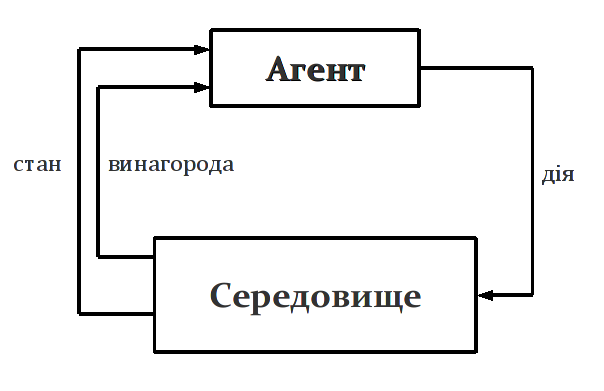
\includegraphics[width=0.5\textwidth]{agent-env-diagram.png}
\caption{Схема взаємодії агента та середовища}
\label{fig:agent-env-diagram}
\end{figure}

Схематично взаємодію агента та середовища представлено на рис.~\ref{fig:agent-env-diagram}. В дискретний момент часу $t$ агент отримує \emph{стан} середовища $s_t \in \mathcal{S}$, на основі цієї інформації він обирає та здійснює певну \emph{дію} $a_t \in \mathcal{A}(s_t)$, в результаті чого отримує \emph{миттєву винагороду} $r_t \in \mathbb{R}$. Метою агента є вироблення такої \emph{стратегії}, яка б кожній можливої ситуації $s_t$ ставила у відповідність таку дію $a_t$, що дає в перспективі максимальну сумарну винагороду (\emph{очікуваний прибуток} $R_t$). Цю стратегію прийнято позначати як функцію $\pi$. В найбільш загальному випадку, коли середовище, в якому повинен діяти агент, є стохастичним, стратегія є відображенням  $\pi:\mathcal{S}\times\mathcal{A} \rightarrow [0,1]$ простору станів та дій на ймовірність того, що дія $a$ для стану $s$ є оптимальною. В більш простих системах, які є детермінованими або стохастичність яких незначна, частіше використовують детерміновану стратегію $\pi:\mathcal{S} \rightarrow \mathcal{A}$, яка ставить у відповідність певному стану системи оптимальну дію в ньому.

Очікуваний прибуток $R_t$ найчастіше визначають кількома способами, найпопулярнішими з яких є наступні:
\begin{enumerate}
	\item $R_t = \sum\limits_{k=0}^{\infty}r_{t+k}$;
	\item $R_t = \sum\limits_{k=0}^{t_{\max}}r_{t+k}$;
	\item $R_t = \sum\limits_{k=0}^{\infty}\gamma^k r_{t+k}$;
\end{enumerate}

Перше визначення очікуваного прибутку можна застосовувати в тих задачах, в яких дія агента може відбуватися як завгодно довго, можливо, навіть неперервно. Друге визначення підходить для задач, в яких дія агента відбувається епізодами зі скінченною кількістю ходів. Більш гнучким та зручним є третє визначення --- зважена нескінченна сума миттєвих винагород. Параметр $\gamma \in [0,1]$ визначає коефіцієнт зважування миттєвих винагород. Його підбором можна гнучко регулювати важливість обраних дій залежно від їх віддаленості у часі. Якщо $\gamma = 0$, то агент є ``недалекоглядним'' і буде дбати лише про максимізацію миттєвої винагороди лише на поточному кроці. При такому $\gamma$ агент буде діяти жадібно і в загальному така стратегія приведе лише до субоптимального очікуваного прибутку. В більшості задач часто буває вигідно на певному кроці здійснити дію, яка не забезпечує максимальної винагороди на даному кроці, зате дає змогу в майбутньому отримати більший сумарний прибуток. З наближенням $\gamma$ до 1 агент надаватиме майбутнім винагородам все більшого значення, а отже його поведінка стає більш ``далекоглядною''. В нашій задачі ми зупинимось на використанні саме зваженого очікуваного прибутку.

Існують різноманітні підходи до навчання агента. Одним з таких підходів є алгоритми які базуються на побудові \emph{функції корисності} $V(s)$, яка визначає максимальний очікуваний прибуток, який можна отримати зі стану $s$ при умові строгого слідування оптимальній стратегії і надалі. Серед цих методів можна виділити три категорії алгоритмів:

\begin{itemize}
\item методи динамічного програмування;
\item методи Монте-Карло;
\item методи часової різниці.
\end{itemize}

В даній статті ми розглянемо алгоритми, що належать до останньої категорії, оскільки перші дві не є надто практичними для більшості реальних застосувань. Для більш детального ознайомлення з цими методами можна звернутися до \cite{SuttonBarto2002}.

При визначенні функції корисності $V(s)$ неявно розуміється, що стратегія згідно якої відбувається вибір оптимальної дії на поточному кроці та на всіх наступних кроках є фіксована. Таким чином, функція корисності визначається по відношенню до певної стратегії $\pi$.

\emph{Корисність} стану $s$ згідно стратегії $\pi$, $V^\pi(s)$,"--- це очікуваний прибуток, який можна отримати, якщо почати зі стану $s$ і діяти надалі строго згідно певної стратегії $\pi$:
\begin{equation}
V^\pi(s) = E_\pi \Bigl\{ R_t \Big| s_t = s \Bigr \} = E_\pi \Biggl\{\sum_{k=0}^{\infty}\gamma^k r_{t+k} \Bigg| s_t=s \Biggr\},
\end{equation}
де $E_\pi{}$ позначає математичне очікування в випадку, якщо агент діє згідно стратегії $\pi$. Потрібно відмітити, що \emph{очікуваний прибуток термінального стану}, тобто стану, при переході в який діяльність агента припиняється і епізод вважається завершеним, завжди рівна нулю. Назвемо функцію $V^\pi$ \emph{функцією корисності станів для стратегії $\pi$}.

Часто використовують розширення функції $V^\pi(s)$, яке виявляється для деяких алгоритмів значно зручнішим та ефективнішим. Визначимо корисність здійснення дії $a$ в стані $s$ згідно стратегії $\pi$, $Q^\pi(s,a)$, як очікуваний прибуток, що можна отримати, здійснивши у стані $s$ дію $a$ та надалі строго притримуючись тієї ж стратегії $\pi$:
\begin{equation}
Q^\pi(s,a)=E_\pi \Bigl\{ R_t \Big| s_t=s, a_t=a \Bigr\} = E_\pi \Biggl\{\sum_{k=0}^{\infty}\gamma^k r_{t+k} \Bigg| s_t=s,a_t=a \Biggr\}.
\end{equation}
Назвемо функцію $Q^\pi$ \emph{функцією корисності дій для стратегії $\pi$}.

Функції корисності $V^\pi$ та $Q^\pi$ в загальному випадку точно визначити неможливо, особливо при неповних даних про модель динаміки системи, проте їх можна оцінити з досвіду. В найпростішому випадку це можна зробити наступним чином. Якщо агент притримується стратегії $\pi$ і для кожного стану зберігає середнє значення прибутку, отриманого в усіх епізодах, що відбулися, то це значення згідно теореми великих чисел збіжиться до математичного очікування корисності для даного стану $V^\pi(s)$ за умови, що середні значення будуть оновлюватися для кожного стану нескінченну кількість разів. Аналогічне твердження справедливе і для функції $Q^\pi$, якщо зберігати середні значення для кожної пари $(s,a)$. Такі методи оцінки функцій корисності лежать в основі методів Монте-Карло, про які ми згадували раніше. Проте, якщо кількість станів та можливих дій велика, вимога нескінченної кількості оновлень для кожного стану стає на заваді точному наближенню функцій корисності.

Функції корисності визначають частковий порядок на множині усіх стратегій. Стратегію $\pi$ називатимемо \emph{кращою}, ніж стратегія $\pi '$, якщо її очікуваний прибуток більший або рівний від такого ж для стратегії $\pi '$ для усіх станів $s \in \mathcal{S}$:
\begin{equation}
\pi \geq \pi ' \Leftrightarrow \Bigl(\forall s \in \mathcal{S}\Bigr)\left\{ V^\pi(s) \geq V^{\pi '}(s) \right\}
\end{equation}

Завжди існує стратегія, яка краща або ж не гірша від усіх інших. Така стратегія називається \emph{оптимальною}. Хоча оптимальних стратегій може бути декілька, всіх їх будемо позначати як $\pi^*$. Усі оптимальні стратегії мають одну і ту ж функцію корисності станів, яка називається \emph{оптимальною функцією корисності станів} $V^*$:
\begin{equation}
V^* = \max_\pi V^\pi(s),\qquad \forall s \in \mathcal{S}.
\end{equation}

Оптимальні стратегії також мають одну і ту ж \emph{функцію корисності дій} $Q^*$:
\begin{equation}
Q^* = \max_\pi Q^\pi(s,a),\qquad \forall s \in \mathcal{S}, \forall a \in \mathcal{A}(s).
\end{equation}

\textit{Завданням алгоритмів навчання, розглянутих нами, є максимально ефективне та точне наближення функції корисності до оптимальної, використовуючи обмежені дані про взаємодію з середовищем.}

\subsection{Навчання з часовою різницею (TD-методи)}

Методи \emph{навчання з часовою різницею (temporal-dіfference, TD-навчання)} "--- це поєднання ідей методів Монте-Карло та динамічного програмування. TD-методи можуть, як і методи Монте-Карло, навчатися лише з досвіду, не потребуючи знання динаміки моделі середовища (це необхідна умова для методів динамічного програмування). З іншого боку, так само як і в методах динамічного програмування, TD-методи оновлюють свої оцінки частково на основі інших оцінок, не чекаючи закінчення епізоду (методи Монте-Карло змушені чекати закінчення епізоду).

Одними з достатньо ефективних на практиці та простих TD-методів навчання є \emph{Q-навчання} та \emph{Sarsa}. Ці алгоритми використовують функцію корисності дій $Q^\pi(s,a)$. В основі їхньої роботи лежить ітераційне почергове наближення стратегії $\pi$ та функції корисності станів $Q^\pi(s,a)$ до оптимальних: $\pi^*$ та $Q^*(s,a)$.

Зупинимось наразі на алгоритмі Sarsa. Будемо розглядати випадок, коли діяльність агента відбувається епізодично, тобто гарантовано за скінченну кількість кроків агент переходить у термінальний стан. Суть алгоритму полягає в наступному. 

Початково довільним чином ініціалізується функція $Q(s,a)$. На початку кожного епізоду агент певним чином (наприклад, випадково) розташовується у середовищі і йому подається початковий стан $s_0$. Після цього агент вибирає найкращу дію $a_0$ для стану $s_0$ на основі значень функції $Q(s_0,a)$. Далі для кожного кроку епізоду агент здійснює обрану дію $a_t$ і отримує від середовища відповідну миттєву винагороду $r_t$ та наступний стан $s_{t+1}$. Знову обирається найкраща дія $a_{t+1}$ для стану $s_{t+1}$. Визначивши усе це, агент оновлює свою функцію корисності згідно наступного правила:
\begin{equation} 
Q(s_t,a_t) \leftarrow Q(s_t,a_t) + \alpha\left[ r_{t+1} + \gamma Q(s_{t+1},a_{t+1}) - Q(s_t, a_t)\right],
\label{eq:sarsa-update-rule}
\end{equation}
де $\alpha \in \mathbb{R}$ --- крок навчання.

Цей процес відбувається доти, доки агент не досягне термінального стану. Після цього починається новий епізод і все починається спочатку. В табл.~\ref{table:Sarsa_algorithm} наведений алгоритм Sarsa.

\begin{table}
\centering
\begin{tabular}{|l|}
\hline\\
Ініціалізувати $Q(s,a)$ довільним чином\\
Для кожного епізоду повторювати:\\
\hspace{0.5cm} $t \leftarrow 0$\\
\hspace{0.5cm} Ініціалізувати $s_t$\\
\hspace{0.5cm} Обрати $a_t$ для стану $s_t$ згідно стратегії, що базується на $Q$ (наприклад, $\varepsilon$-жадібної)\\
\hspace{0.5cm} Повторювати для кожного кроку епізоду:\\
\hspace{1cm} 	Здійснити дію $a_t$, отримати $r_t$, $s_{t+1}$\\
\hspace{1cm} 	Обрати $a_{t+1}$ для стану $s_{t+1}$ згідно обраної стратегії\\
\hspace{1cm} 	$Q(s_t,a_t) \leftarrow Q(s_t,a_t) + \alpha\left[r_t + \gamma Q(s_{t+1},a_{t+1}) - Q(s_t,a_t)\right]$\\
\hspace{1cm} 	$t \leftarrow t + 1$\\
\hspace{0.5cm} поки $s_t$ "--- не термінальний стан\\
\\
\hline
\end{tabular}
\caption{Алгоритм Sarsa.}
\label{table:Sarsa_algorithm}
\end{table}

Алгоритм Q-навчання є дуже схожим до Sarsa і відрізняється лише у правилі оновлення значення функції корисності $Q$:
\begin{equation}
Q(s_t,a_t) \leftarrow Q(s_t, a_t) + \alpha \left[ r_t + \gamma \max_{a \in \mathcal{A}(s_t)} Q(s_{t+1}, a) - Q(s_t,a_t) \right].
\label{eq:q-update-rule}
\end{equation}

Q-навчання добре розроблене в теоретичному плані, існують теореми, які доводять, що наближення Q-функції у границі при нескінченній кількості взаємодій з середовищем та нескінченній кількості оновлень кожної можливої пари $(s_t,a_t)$ збігаються до оптимальної $Q^*$-функції. 

Q-навчання є дуже простим для розуміння та теоретично обґрунтованим, проте часто на практиці значно краще себе показує алгоритм Sarsa, який проте не має настільки хорошого теоретичного підґрунтя. Слід зазначити, що після достатньої кількості ітерацій навчання, коли значення Q-функції вже не будуть настільки випадково розподіленими, як на початку навчання, дія $a_{t+1}$ на наступному кроці все частіше буде оптимальною. Таким чином, оновлення для Q- та Sarsa-навчання з часом будуть відбуватися однаково. Але при цьому Sarsa-навчання на практиці часто забезпечує швидшу збіжність Q-функції до оптимальної.

\subsection{Стратегії вибору дій}
В розглянутих алгоритмах потрібно на кожному кроці здійснювати вибір дії, яку повинен виконати агент. Це можна робити різними способами, проте, для збіжності стратегії до оптимальної, необхідною умовою є те, щоб кожна можлива дія була випробувана безліч раз при умові безмежної кількості ітерацій. Таку умову задовольняють так звані soft-стратегії, в яких ймовірність вибору кожної дії для будь-якого стану є ненульовою:
\[
\pi(s,a)>0,\ \forall \pi, \forall s \in \mathcal{S}, a \in \mathcal{A}(s).
\]

Одним з найпростіших випадків soft-стратегії є $\varepsilon$-жадібна стратегія. В такій стратегії з ймовірністю $1-\varepsilon$ вибирається дія, що забезпечує максимум функції корисності, а з ймовірністю $\varepsilon$ --- випадкова допустима дія. Таким чином будь-яка не жадібна дія виконується з ймовірністю $\dfrac{\varepsilon}{|\mathcal{A}(s)|}$, а ``жадібна'' --- з ймовірністю $1 - \varepsilon + \dfrac{\varepsilon}{|\mathcal{A}(s)|}$.

\subsection{Труднощі у випадку неперервного простору станів}

Якщо множина станів системи $\mathcal{S}$ дуже велика, як у випадку багатьох класичних ігор, або ж неперервна, що часто трапляється, наприклад, в робототехніці, то постає складне питання представлення функцій корисності. Існує багато варіантів вирішення цієї проблеми. І хоч ефективність кожного з методів сильно залежить від конкретної задачі, одним з найбільш універсальних методів є лінійні та нелінійні апроксиматори функцій. При цьому лінійні апроксиматори, хоч і менш гнучкі та потужні, проте в більшості задач чудово справляються зі своїми завданнями. Більше того, існують теоретичні гарантії збіжності до оптимальної стратегії для алгоритмів Sarsa та Q-навчання у випадку використання лінійних апроксиматорів функцій, якщо останні задовольняють певні умови (\cite{Coulom2002}).

У випадку з нелінійними апроксиматорами, такими як штучні нейронні мережі, ситуація не настільки визначена. Загалом немає ніяких гарантій успішної збіжності до оптимальних стратегій. Більше того, для певних задач було доведено розбіжність розглянутих нами алгоритмів при використанні нейромереж в якості апроксиматора функції корисності (більш детальну інформацію можна знайти в \cite{SuttonBarto2002}). Тим не менше, нейромережі все ж таки успішно використовуються у різноманітних алгоритмах навчання з підсиленнями. Більше того, здатність нейромереж до узагальнення дає можливість швидше навчати агента, оскільки визначивши вартість певного стану, вона наближає і вартості близьких до нього станів. Таким чином можна надіятись на швидшу збіжність стратегії до оптимальної.

У нашому випадку також була використана нейромережа як апроксиматор функцій і, як буде видно з результатів, досить успішно.

\subsection{Постановка задачі для підходу на основі навчання з підсиленням}

Для того, щоб більш ефективно використати навчання з підсиленням, були внесенні певні модифікації в формулювання задачі. Так, завдання агента було ускладнене "--- вимагалося, щоб агент не тільки оминав перешкоди, але й добирався до заданої цілі.

При цьому, щоправда, були деякі спрощення: час вважався дискретним, була спрощена фізика автомобіля. Тепер було можливо робити розворот на місці, що дозволяло уникнути певних проблем, з якими ми зіткнулися у попередньому підході. Також було дещо спрощено керування агентом: тепер були доступні лише п'ять дій.

\begin{figure}
  \centering
  \subfloat[Віртуальне середовище]
  {
	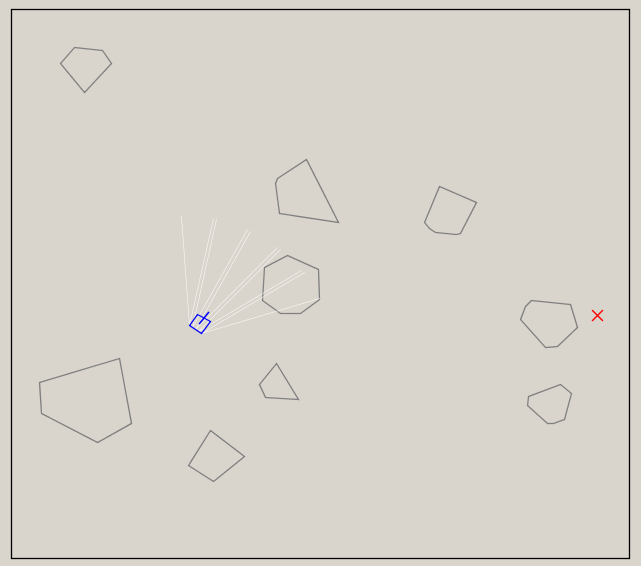
\includegraphics[width=0.33\textwidth]{env-screen.png}
	\label{fig:environment}
  }\,
  \subfloat[Сприймання агентом середовища]
  {
  	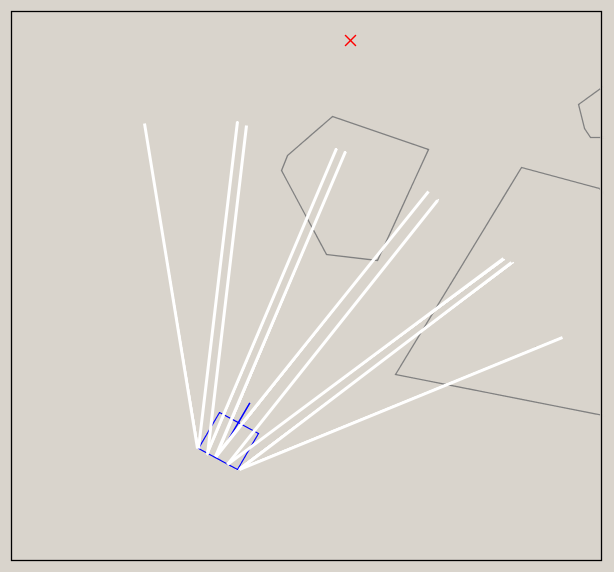
\includegraphics[width=0.31\textwidth]{perception}
  	\label{fig:perception}
  }\,
  \subfloat[Невдалий варіант зони сприймання]{
  	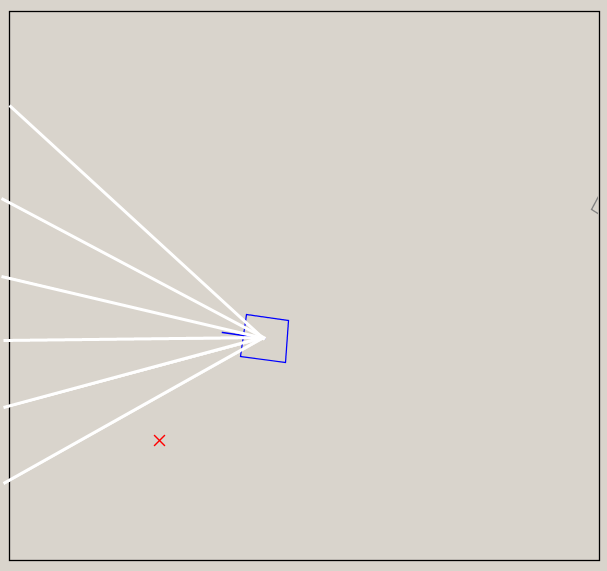
\includegraphics[width=0.31\textwidth]{bad-perception} 
    \label{fig:bad-perception}
  }
  \caption{Ілюстрації до другого підходу}
  \label{fig:second-approach}
\end{figure}

Для випробування на практиці навчанням з підсиленням в застосуванні до задачі керування автономним агентом було створено віртуальне середовище (див. рис.~\ref{fig:environment}), в якому і відбувалися усі практичні експерименти. Середовище становить собою квадратну кімнату, в якій знаходяться випадково згенеровані та розташовані перешкоди --- опуклі многокутники. Уся дія відбувається епізодами. Агент починає на початку кожного епізоду свій рух у випадковій позиції з випадковим початковим напрямом руху і повинен дістатися вказаної точки, яка також генерується випадково. При цьому першочерговою вимогою є те, що агент повинен добратися до цілі без зіткнень з перешкодами та межами кімнати, другорядною --- добирання до цілі повинно бути якомога швидшим.

Вхідні дані, які надавалася агенту, були дещо розширені. Секторів огляду в агента стало 5, при цьому розміщувалися вони так, як показано на рис.~\ref{fig:perception}. Таке розташування дає змогу сприймати об'єкти, що знаходяться дуже близько збоку, що покращує поведінку агента. Також агенту надавалася інформація про відстань до цілі та кут між напрямом руху агента та напрямком на ціль. 

Для навчання використовувався алгоритм Sarsa. В якості стратегії вибору дій була вибрана $\varepsilon$-жадібна стратегія. Параметр $\gamma$ було прийнято рівним $0.99$ для того, щоб зробити рух агента більш оптимальним в довгостроковій перспективі.

Агенту були доступні 5 можливих дій:
\begin{itemize}
	\item рухатись прямо на фіксовану відстань;
	\item рухатись прямо на фіксовану відстань, одночасно повернувши наліво на фіксований кут повороту;
	\item рухатись прямо на фіксовану відстань, одночасно повернувши направо на фіксований кут повороту;
	\item залишитися на місці, повернувши наліво на фіксований кут повороту;
	\item залишитися на місці, повернувши направо на фіксований кут повороту.
\end{itemize}

Рух робота продовжується доти, доки не буде виконана одна з наступних умов:
\begin{itemize}
	\item досягнуто цілі;
    \item зіткнення з перешкодою або межею кімнати;
	\item перевищено ліміт кількості кроків (таймаут);
\end{itemize}

В усіх цих випадках епізод вважається закінченим. В результаті, залежно від того, яка саме умова спричинила закінчення епізоду, агенту надається певна винагорода. Після цього знову генерується випадковий епізод і все повторюється з початку. 

Нагадаємо, що для навчання з підсиленням потрібно визначити систему винагород, яка визначає яку винагороду отримує агент при переході з одного стану у інший. Нами була вибрана наступна система винагород:
\begin{itemize}
	\item при досягненні кінцевої цілі надавалася винагорода, рівна $1.00$. Це є набільшою миттєвою винагородою і повинно сприяти досягненню агентом кінцевої цілі;
	\item при зіткненні з перешкодою: $-1 + \frac{1}{2} e^{-2\frac{d_{crash}}{d_{size}}}$, де $d_{crash}$ --- відстань між місцем зіткнення з перешкодою та кінцевою ціллю агента; $d_{size}$ --- довжина сторони кімнати. Ця винагорода є мінімальною, а отже зіткнення --- найменш бажана подія;
	\item при перевищенні ліміту дозволених кроків агенту видавалася така ж винагорода, як і у випадку зіткнення, проте більша на $0.3$. Це також небажана подія, проте безпечне пересування є більш пріоритетним, аніж зіткнення з перешкодою;
	\item в усіх інших випадках миттєва винагорода становила $-0.01$. Цим досягалося те, що агент намагався (неявно) мінімізувати кількість кроків до досягнення цілі.
\end{itemize}

Усі вхідні дані --- дійсні числа, тому ми змушені були боротися з неперервним простором станів. Для цього в якості апроксиматора функції корисності ми використали нейромережу прямого поширення, яка на кожній ітерації навчалася одним проходом алгоритму зворотнього поширення похибки. В усіх прошарках нейромережі в якості активаційної функції використовувалася логістична функція ($f(x) = \frac{1}{1 + e^{-x}}$), в останньому вихідному прошарку --- одинична ($f(x) = x$).

Для апроксимації функції $Q(s,a)$ використовувалися 5 окремих нейромереж, кожна з яких відповідала за свою дію. Цей підхід, згідно \cite{Rummery1995}, є ефективнішим, ніж використання однієї нейромережі з кількістю виходів, рівною кількості можливих дій. В такому випадку для роботи нейромережі достатньо меншої кількості ітерацій навчання, а також меншої кількості нейронів.

На вхід нейромережі подавалися спеціальним чином закодовані 7 відомих параметрів стану: 5 значень відстаней для кожного з секторів поля зору, а також відстань до цілі та кут. Спосіб кодування був взятий з \cite{Rummery1995}. Експерименти показали, що таке кодування вхідних даних суттєво полегшує задачу навчання нейромережі і робить його ефективнішим та якіснішим.

Усі вагові коефіцієнти нейромережі були початково ініціалізовані нулями, що завдяки одиничній функції у вихідному прошарку, початково давало значення нуль для будь-якого входу. Це є досить важливим моментом. В літературі (\cite{SuttonBarto2002}) рекомендують при можливості використовувати таке початкове наближення функції корисності $Q(s,a)$, яке б було оптимістичним, по відношенню до реальної функції вартості. В такому випадку агент, вибравши певну дію і отримавши винагороду, яка є нижчою, ніж початкове оптимістичне наближення, наступного разу в тій же ситуації буде схилятися до вибору іншої дії, таким чином пробуючи кожного разу іншу дію. Таке початкове випробування усіх можливих дій забезпечує швидше та більш точне наближення реальної функції корисності. 

Агент на перших стадіях навчання діє дуже неефективно. Оскільки ймовірність добратися до цілі, минаючи перешкоди, в умовах випадково згенерованого середовища дуже невелика, то початково постійно буде отримуватися негативне значення винагороди. Тому нульова ініціалізація нейромережі становить собою оптимістичні сподівання, і, відповідно, є корисною евристикою.

\subsection{Результати}

Практичні експерименти показали, що зазвичай агенту достатньо $1.2$ мільйонів кроків навчання для того, щоб розробити ефективну власну стратегію, після чого вона практично не змінюється. Ефективність контролера оцінювалася у відсотках успішних добирань до цілі за останні $5000$ епізодів, щоб знівелювати вплив фактично випадкових дій на початку навчання.

Початково значення $\varepsilon$ у $\varepsilon$-жадібній стратегії було фіксованим на позначці $0.1$, що становило собою розумний компроміс між випадковістю поведінки та можливістю дослідження ``нерозвіданих'' дій. При цьому вершини секторів області сприймання починалися у центральній точці робота. Таке поєднання налаштувань дозволяло агенту досягати успішності в $60\%-65\%$ випадків. При цьому робот поводив себе цілком адекватно, стараючись оминути перешкоди, проте часто зачіпаючи боковою стороною краї перешкоди. Це зумовлено обмеженістю поля зору (рис.~\ref{fig:bad-perception}), оскільки сектори захоплювали лише ту частину простору, яка знаходилася безпосередньо перед роботом, ніяк не даючи знати про перешкоди, що знаходяться близько ліворуч та праворуч.

Для того, щоб дати більше інформації про оточуючі перешкоди, поле зору робота було дещо видозмінене (див. рис.~\ref{fig:perception}). Вершини секторів були зміщені в задню частину і рівномірно розподілені по всій задній стороні. Таким чином, у робота тепер були два сектори, які надавали йому інформацію про дуже близькі перешкоди, що знаходилися ліворуч та праворуч від нього. Ці вдосконалення дозволили підвищити успішність агента до позначки $80\%-82\%$ в більшості тестових запусків. Аналіз нової стратегії показав, що поведінка робота дійсно стала значно безпечнішою та ефективнішою. Але при цьому часто можна було спостерігати як робот оминає перешкоду, об'їжджаючи її ``впритул'', і час від часу здійснює випадкові повороти в сторону перешкоди. Це було зумовлено тим, що значення ймовірності вибору випадкової дії $\varepsilon$ було вибрано досить великим "--- $0.1$. Тобто в середньому в одному випадку з десяти агент здійснював випадковий вибір дії, що призводило до зіткнень при близькості до перешкоди.

Зменшення $\varepsilon$ до $0.01$ призвело до значного погіршення навчального процесу, оскільки алгоритму Sarsa не надавалося достатньої можливості досліджувати нові стратегії, натомість поведінка агента збігалася до субоптимальної стратегії.

В результаті цих спостережень ми вирішили використати змінний показник $\varepsilon$, який лінійно спадав від $0.2$ до $0.01$ протягом 1 мільйону кроків навчання, після чого фіксувався на мінімальній позначці. Таке вдосконалення повинно було б допомогти агенту на початку дослідження більш повно досліджувати можливі невипробувані дії, при цьому зменшуючи ймовірність вибору неоптимальних дій тоді, коли в результаті багатьох ітерацій, вивчена функція цінності давала хороше уявлення про оптимальні дії і необхідність додаткового дослідження зменшувалася.

Експеримент показав, що таке вдосконалення дійсно дає краще результати. З усіма вищезазначеними вдосконаленнями в 8 випадках із 10 успішність агента становила $87\%-92\%$ успішних епізодів. В інших 2 випадках з 10, на жаль, агент виробляв стратегію, яка дуже часто просто зациклювала робота на місці, оскільки добратися агент до цілі не міг, то ефективнішим варіантом було залишатися на місці і отримати винагороду все ж вищу, ніж при зіткненні.

Для того, щоб сформувати певне уявлення про еволюцію поведінки агента, розглянемо (рис.~\ref{fig:learning-samples}) рух агента в межах однієї й тієї ж конфігурації перешкод та початкових умов на різних стадіях навчання. На цих ілюстраціях символом + позначено рух робота, + в квадраті "--- фінальна позиція робота, + в крузі "--- початкова позиція робота, x "--- ціль.

Як бачимо, без будь-якого навчання рух агента зовсім випадковий. Після 100 тис. ітерацій агент намагається рухатися в напрямку до цілі, ігноруючи будь-які перешкоди. Після 500 тис. ітерацій агент будь-якою ціною намагається уникнути зіткнення, але при цьому перевищує ліміт дозволених кроків і не добирається до цілі. Після 1.2 млн ітерацій, як видно з рисунка, агент рухається якомога оптимальнішою траєкторією в напрямку до цілі, при цьому досить віртуозно оминаючи перешкоди.
\begin{figure}
  \centering
  \subfloat[Без навчання]{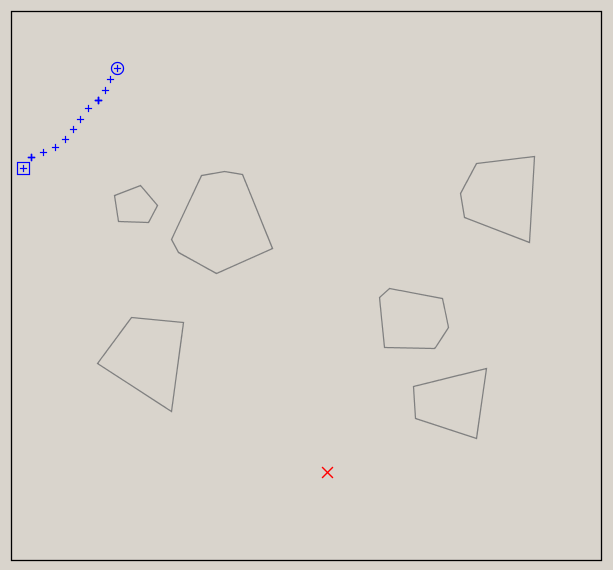
\includegraphics[width=0.47\textwidth]{learn1}}\,
  \subfloat[Після $100$ тис. ітерацій]{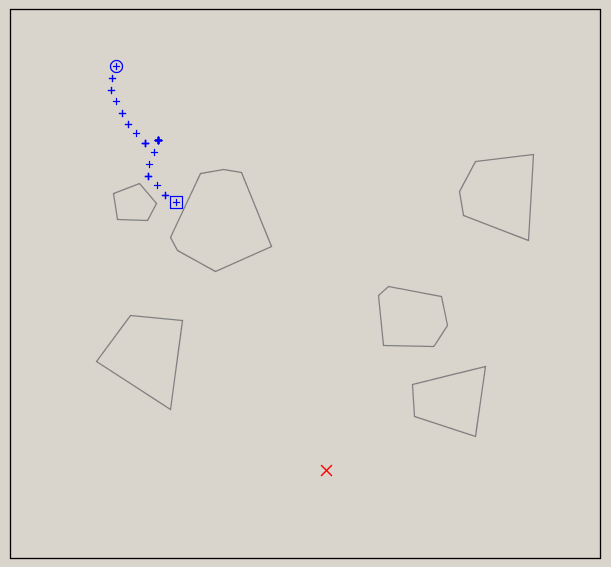
\includegraphics[width=0.47\textwidth]{learn2}} \\
  \subfloat[Після $500$ тис. ітерацій]{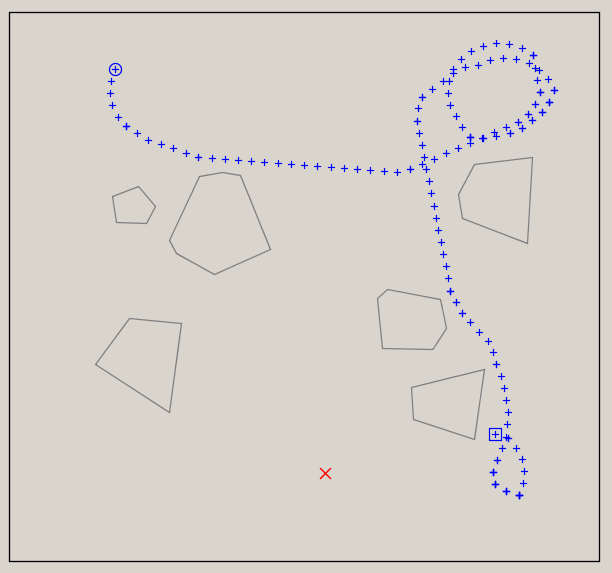
\includegraphics[width=0.47\textwidth]{learn3}}\,
  \subfloat[Після $1.2$ млн. ітерацій]{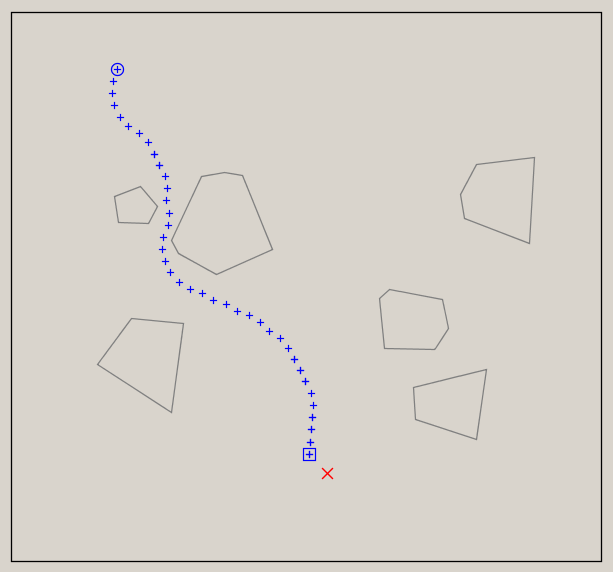
\includegraphics[width=0.47\textwidth]{learn4}}
  \caption{Приклади траєкторій в умовах одного і того ж середовища}
  \label{fig:learning-samples}
\end{figure}

\subsection{Вплив структури та параметрів нейромережі та $\varepsilon$-функції на навчання}

Початково ми проводили усі експерименти з параметрами нейромережі та алгоритму навчання, описаними вище. При цьому у всіх експериментах ми використовували нейромережу, яка складалася з трьох прошарків, в першому розташовувалися 13 нейронів, в другому --- 8, в останньому вихідному --- один нейрон, який мав одиничну активаційну функцію і забезпечував лінійну комбінацію виходів попереднього прошарку. 

Згодом ми вирішили дослідити вплив на ефективність та стабільність результатів навчання структури нейромережі та $\eta$-функції кроку навчання, яка застосовується при навчанні нейромережі за допомогою зворотнього поширення похибки. Також було очевидним, що суттєвий вплив має вигляд $\varepsilon$-функції у $\varepsilon$-жадібній стратегії вибору дій, яку ми використовували. 

Для тестування були обрані наступні функції, яким ми для зручності дали умовні назви:
\begin{itemize}
\item $\eta$-функція кроку навчання нейромережі:
	\begin{itemize}
	\item \textit{eta-linear} --- лінійно-спадна від 0.3 до 0.01 за 600000 ітерацій;
	\item \textit{eta-exp} --- експоненційно-спадна від 0.4 до 0.01 за 600000 ітерацій  (рис.~\ref{fig:eta-exp});
	\item \textit{eta-spikes} --- пилкоподібна з чотирма ``зубцями'', яка спадає від 0.4 до 0.01 за 600000 ітерацій  (рис.~\ref{fig:eta-spikes}).
	\end{itemize}
\item $\varepsilon$-функція:
	\begin{itemize}
	\item \textit{eps-linear} --- лінійно-спадна від 0.3 до 0.0 за 300000 ітерацій;
	\item \textit{eps-spikes} --- пилкоподібна з чотирма ``зубцями'', яка спадає від 0.3 до 0.01 за 300000 ітерацій (аналогічна до \textit{eta-spikes}).
	\end{itemize}
\end{itemize}

\begin{figure}[h]
  \centering
  \subfloat[Експоненційна]{\label{fig:eta-exp}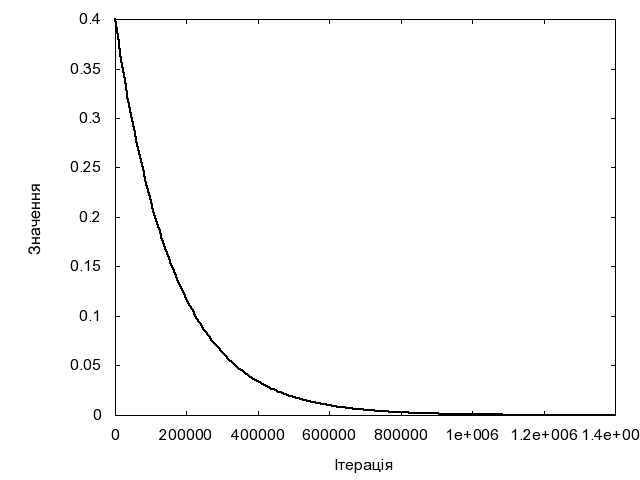
\includegraphics[width=0.4\textwidth]{function-exp}}\,\,\,
  \subfloat[Пилкоподібна]{\label{fig:eta-spikes}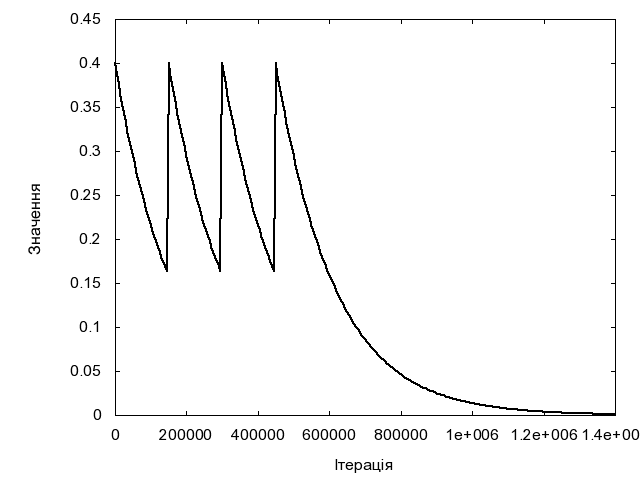
\includegraphics[width=0.4\textwidth]{function-spikes}}
  \caption{Функції}
\end{figure}

Ми провели тести з усіма можливими комбінаціями вищезазначених функцій для двох структур нейромережі: 10-6-1 та 7-4-1. Далі розглянемо ті, які на нашу думку, заслуговують на увагу. Для кожної розглянутої трійки параметрів (структура нейромережі, $eta$- та $\varepsilon$-функції) наведені три графіки, на яких показані кількості епізодів у відсотках від останніх 5000, які закінчились, відповідно, успішним досягненням цілі, зіткненням з перешкодою та перевищенням ліміту дозволених кроків у епізоді. Кожна крива на рисунку відповідає одному з трьох тестових запусків.

\begin{itemize}
\item Нейромережа: 10-6-1, $\eta$-функція: \textit{eta-spikes}, $\varepsilon$-функція: \textit{eps-linear} (рис.~\ref{fig:10-6-spikes-linear}). Цей випадок аналогічний до усіх інших, які ми тут не будемо розглядати. Як бачимо, два з трьох тестових запусків досягають високої успішності, проте третій показує, що така комбінація параметрів не забезпечує належної стабільності результатів, тому що в третьому тестовому запуску агент ``зривається'' на стратегію, яка віддає перевагу таймауту. Така ситуація притаманна більшості досліджених нами комбінацій параметрів.

\begin{figure}[h!]
  \centering
  \subfloat[Успіх]{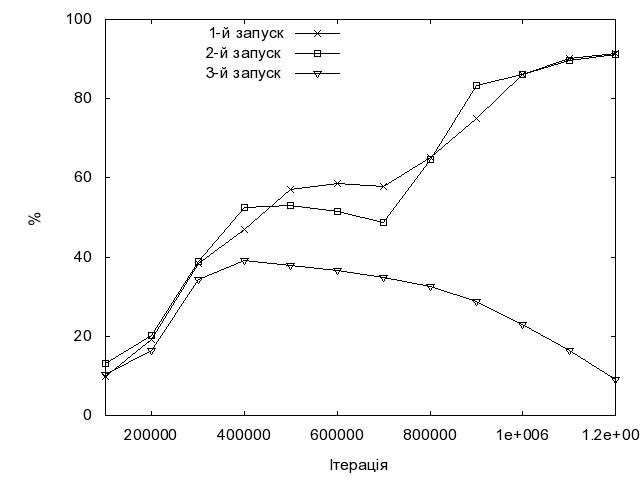
\includegraphics[width=0.3\textwidth]{10-6-spikes-linear_r}}\,
  \subfloat[Зіткнення]{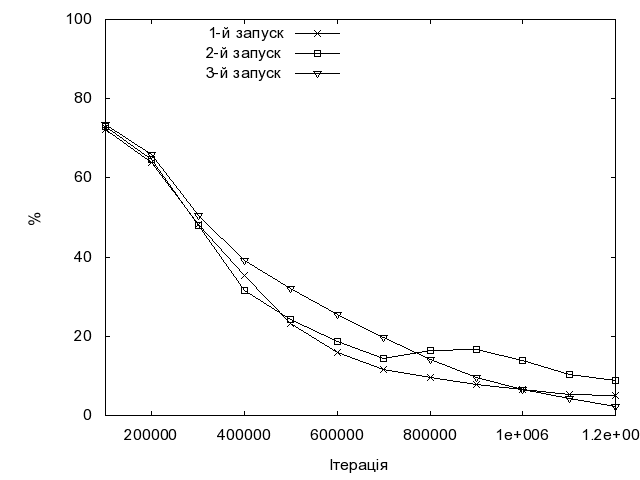
\includegraphics[width=0.3\textwidth]{10-6-spikes-linear_c}}\,
  \subfloat[Таймаут]{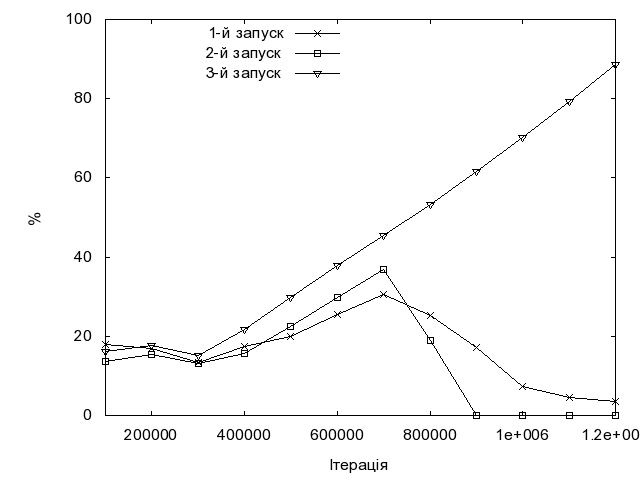
\includegraphics[width=0.3\textwidth]{10-6-spikes-linear_t}}
  \caption{Нейромережа: 10-6-1, eta-spikes, eps-linear}
  \label{fig:10-6-spikes-linear}
\end{figure}

\item Нейромережа: 7-4-1, $\eta$-функція: \textit{eta-spikes}, $\varepsilon$-функція: \textit{eps-linear} (рис.~\ref{fig:7-4-spikes-linear}). Як бачимо, аналогічна поведінка, як і у попередньому випадку, незалежно від конфігурації нейромережі.

\begin{figure}[h!]
  \centering
  \subfloat[Успіх]{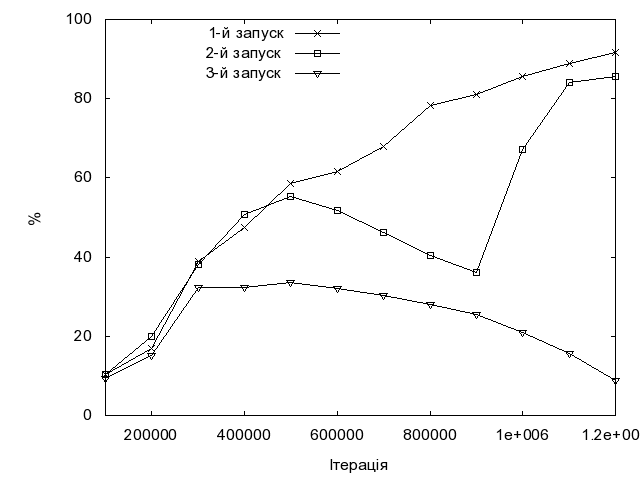
\includegraphics[width=0.3\textwidth]{7-4-spikes-linear_r}}\,  \subfloat[Зіткнення]{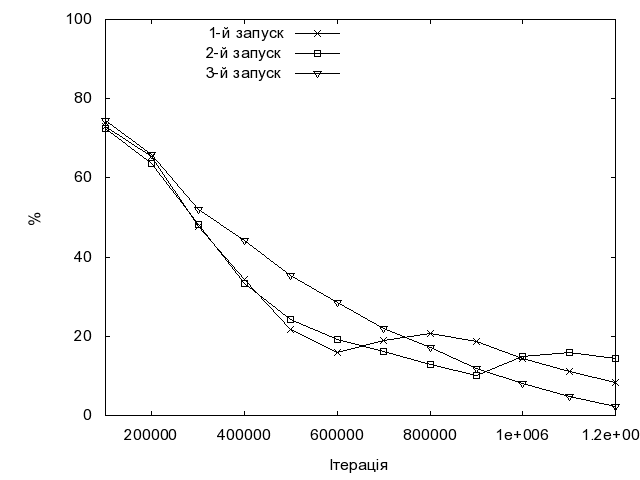
\includegraphics[width=0.3\textwidth]{7-4-spikes-linear_c}}\,
  \subfloat[Таймаут]{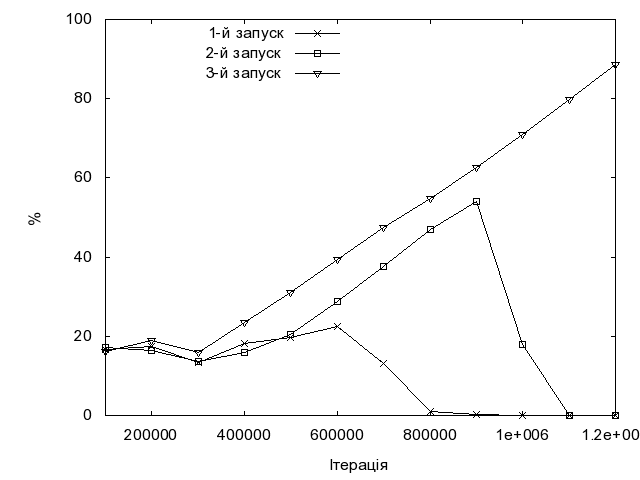
\includegraphics[width=0.3\textwidth]{7-4-spikes-linear_t}}
  \caption{Нейромережа: 7-4-1, eta-spikes, eps-linear}
  \label{fig:7-4-spikes-linear}
\end{figure}

\item Нейромережа: 10-6-1, $\eta$-функція: \textit{eta-spikes}, $\varepsilon$-функція: \textit{eps-spikes} (рис.~\ref{fig:10-6-spikes-spikes}). Ця комбінація параметрів показує себе дуже добре, забезпечуючи стабільне успішне навчання і порівняно високу швидкість збіжності. При цьому слід відзначити наскільки схожі графіки усіх трьох тестових запусків, що ще більше підтверджує хороші характеристики стабільності цієї комбінації.

\begin{figure}[h!]
  \centering
  \subfloat[Успіх]{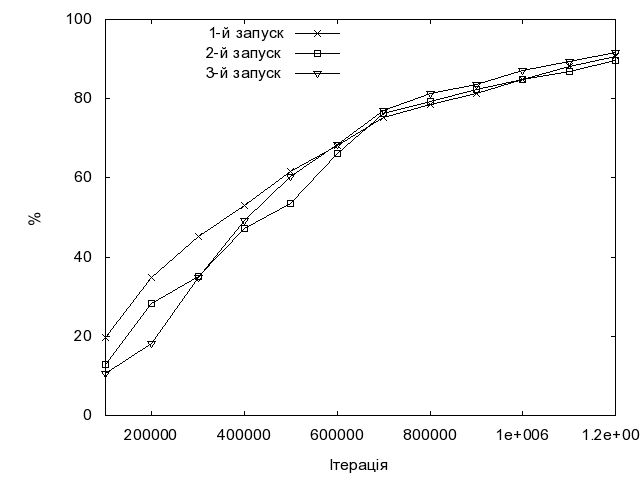
\includegraphics[width=0.3\textwidth]{10-6-spikes-spikes_r}}\,
  \subfloat[Зіткнення]{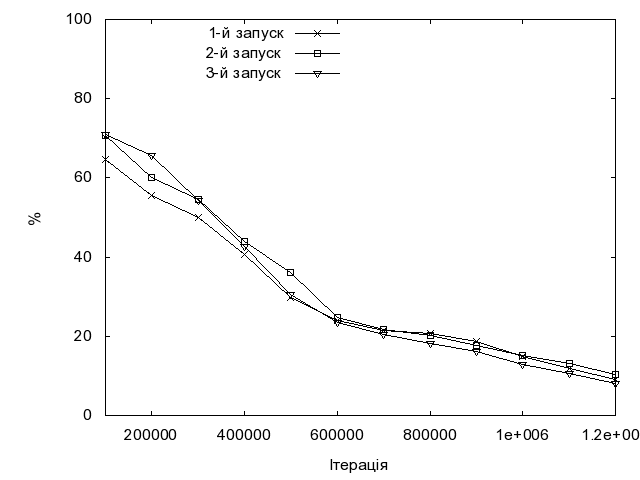
\includegraphics[width=0.3\textwidth]{10-6-spikes-spikes_c}}\,
  \subfloat[Таймаут]{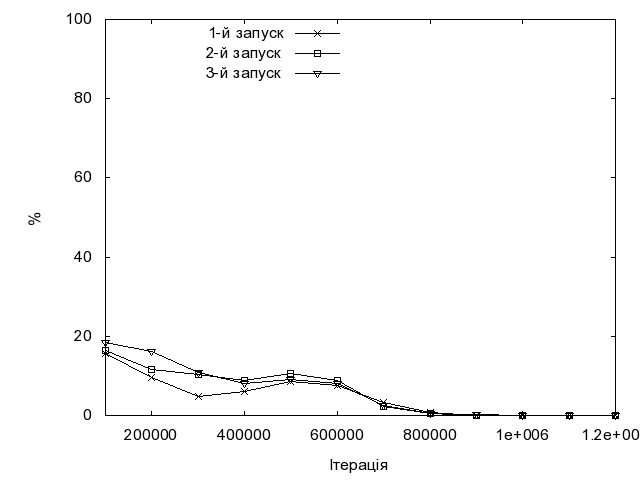
\includegraphics[width=0.3\textwidth]{10-6-spikes-spikes_t}}
  \caption{Нейромережа: 10-6-1, eta-spikes, eps-spikes}
  \label{fig:10-6-spikes-spikes}
\end{figure}

\item Нейромережа: 10-6-1, $\eta$-функція: \textit{eta-exp}, $\varepsilon$-функція: \textit{eps-spikes} (рис.~\ref{fig:10-6-exp-spikes}). Аналогічно до попередньої ситуації хороша стабільність та висока ефективність навченого агента, щоправда на початкових етапах навчання можна спостерігати досить значні відмінності у графіках. Щоправда після того, як вибрані $\eta$- та $\varepsilon$-функції досягають своїх мінімальних значень, ситуація з часом вирівнюється.

\begin{figure}[h!]
  \centering
  \subfloat[Успіх]{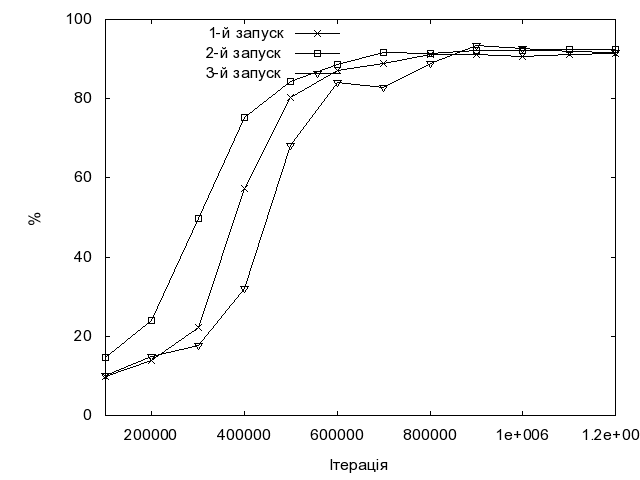
\includegraphics[width=0.3\textwidth]{10-6-exp-spikes_r}}\,
  \subfloat[Зіткнення]{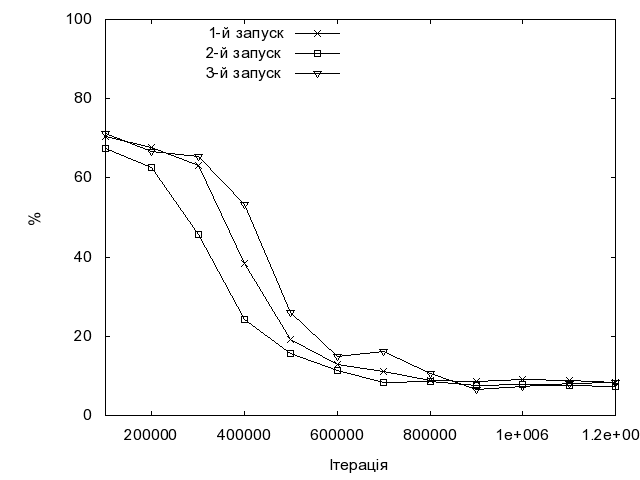
\includegraphics[width=0.3\textwidth]{10-6-exp-spikes_c}}\,
  \subfloat[Таймаут]{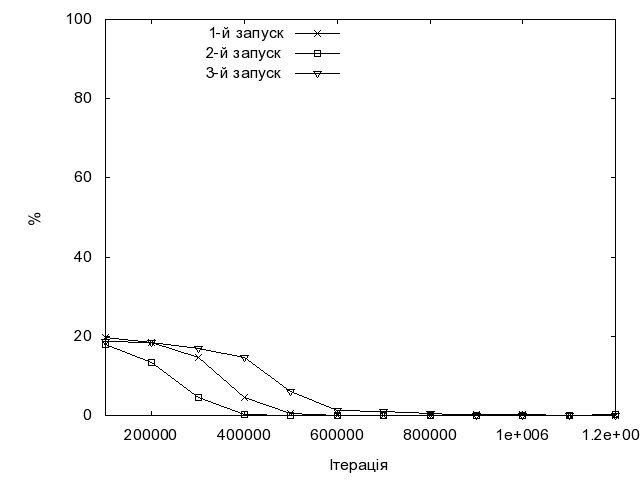
\includegraphics[width=0.3\textwidth]{10-6-exp-spikes_t}}
  \caption{Нейромережа: 10-6-1, eta-exp, eps-spikes}
  \label{fig:10-6-exp-spikes}
\end{figure}

\item Нейромережа: 7-4-1, $\eta$-функція: \textit{eta-spikes}, $\varepsilon$-функція: \textit{eps-spikes} (рис.~\ref{fig:7-4-spikes-spikes}). Аналогічно як і у випадку з більшою структурою нейромережі, хороша стабільність та висока ефективність агента.

\begin{figure}[h!]
  \centering
  \subfloat[Успіх]{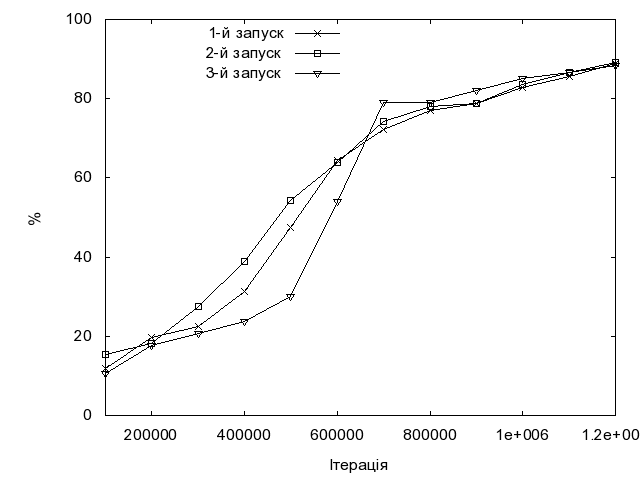
\includegraphics[width=0.3\textwidth]{7-4-spikes-spikes_r}}\,
  \subfloat[Зіткнення]{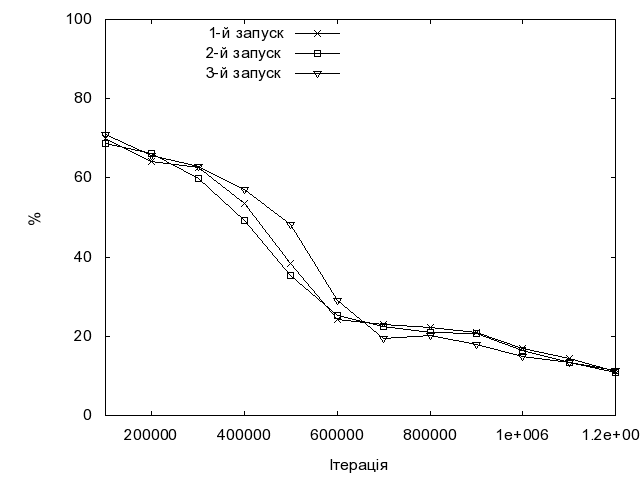
\includegraphics[width=0.3\textwidth]{7-4-spikes-spikes_c}}\,
  \subfloat[Таймаут]{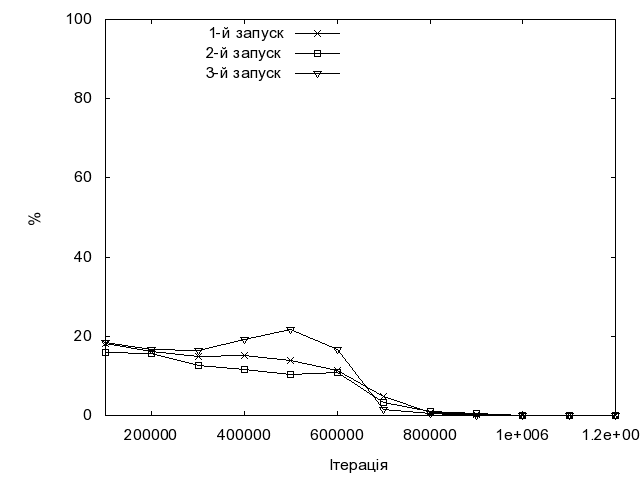
\includegraphics[width=0.3\textwidth]{7-4-spikes-spikes_t}}
  \caption{Нейромережа: 7-4-1, eta-spikes, eps-spikes}
  \label{fig:7-4-spikes-spikes}
\end{figure}

\item Нейромережа: 7-4-1, $\eta$-функція: \textit{eta-exp}, $\varepsilon$-функція: \textit{eps-spikes} (рис.~\ref{fig:7-4-exp-spikes}). Тут ситуація дещо відрізняється від схожої комбінації для нейромережі структури 10-6-1. Ми можемо спостерігати значні розбіжності в ефективності агента, щоправда, якщо продовжити навчання далі, графіки ефективності агента зблизяться.

\begin{figure}[h!]
  \centering
  \subfloat[Успіх]{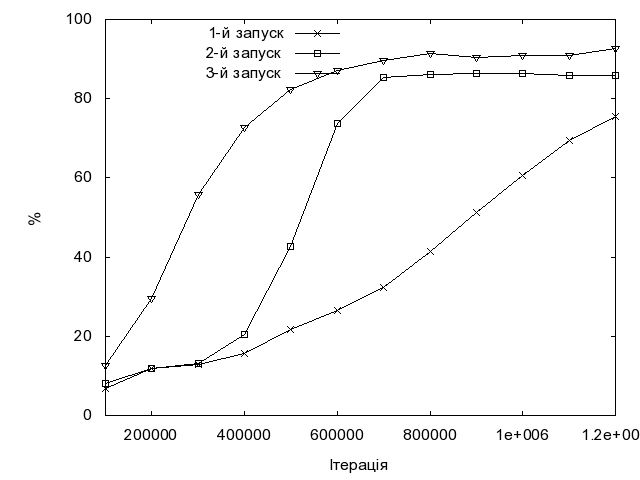
\includegraphics[width=0.3\textwidth]{7-4-exp-spikes_r}}\,
  \subfloat[Зіткнення]{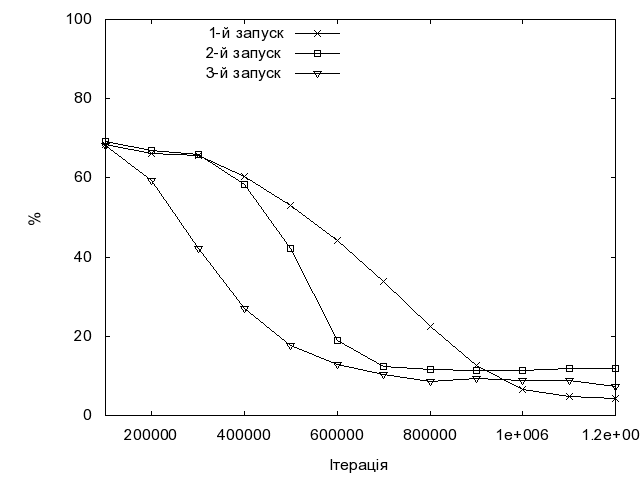
\includegraphics[width=0.3\textwidth]{7-4-exp-spikes_c}}\,
  \subfloat[Таймаут]{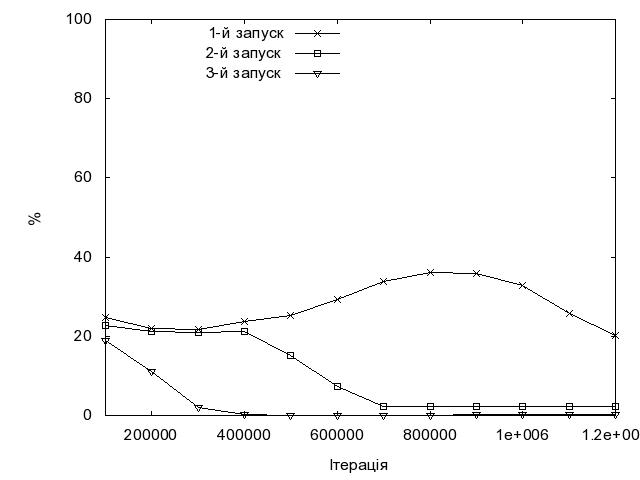
\includegraphics[width=0.3\textwidth]{7-4-exp-spikes_t}}
  \caption{Нейромережа: 7-4-1, eta-exp, eps-spikes}
  \label{fig:7-4-exp-spikes}
\end{figure}

\item Нейромережа: 7-4-1, $\eta$-функція: \textit{eta-linear}, $\varepsilon$-функція: \textit{eps-linear} (рис.~\ref{fig:7-4-linear-linear}). Ця комбінація виявилася дуже хорошою для нейромережі структури 7-4-1, хоча аналогічна комбінація функцій для більшої нейромережі поводила себе нестабільно. Очевидно, зіграло роль те, що лінійна $\eta$-функція у випадку більшого розміру нейромережі призводить до її самозбудження і робить навчання невдалим. Також помітно наскільки близькими є графіки успішності агента, а отже і стабільність даної комбінації функцій. 

\begin{figure}[h!]
  \centering
  \subfloat[Успіх]{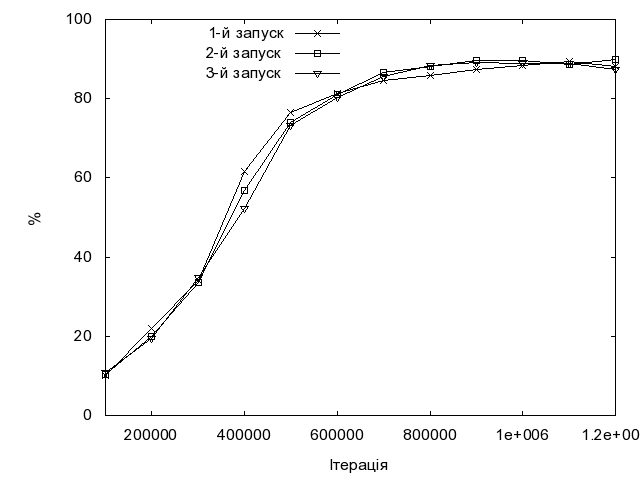
\includegraphics[width=0.3\textwidth]{7-4-linear-linear_r}}\,
  \subfloat[Зіткнення]{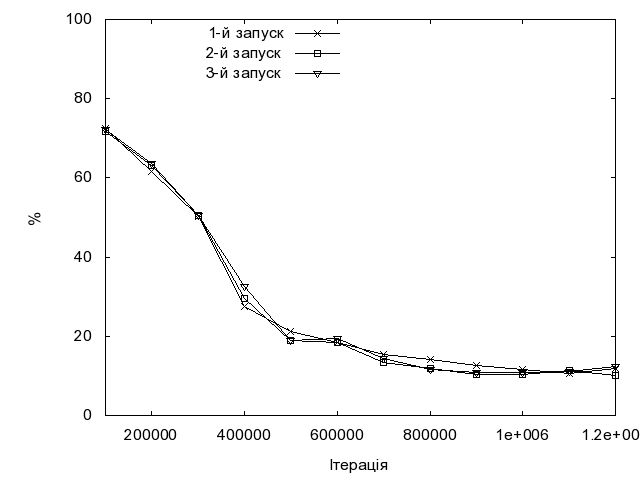
\includegraphics[width=0.3\textwidth]{7-4-linear-linear_c}}\,
  \subfloat[Таймаут]{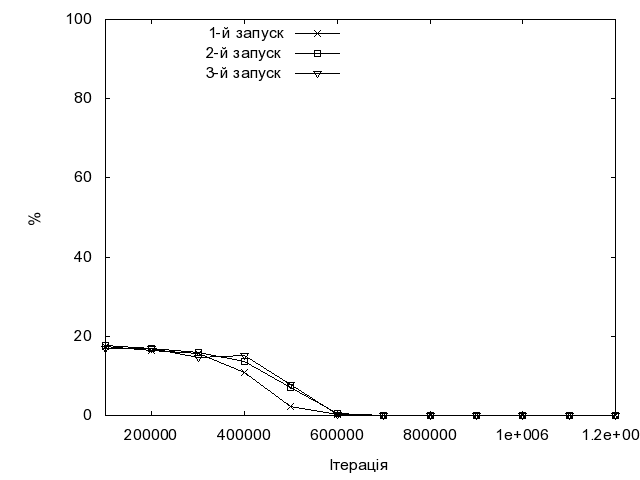
\includegraphics[width=0.3\textwidth]{7-4-linear-linear_t}}
  \caption{Нейромережа: 7-4-1, eta-linear, eps-linear}
  \label{fig:7-4-linear-linear}
\end{figure}

\item Нейромережа: 7-4-1, $\eta$-функція: \textit{eta-linear}, $\varepsilon$-функція: \textit{eps-spikes} (рис.~\ref{fig:7-4-linear-spikes}). Практично ідентична до попередньої ситуація. З цієї та попередньої комбінації видно, що в даних випадках $\varepsilon$-функція стратегії не має жодного впливу на навчання, що ще раз підкреслює виняткову важливість правильної настройки нейромережі та її параметрів.
\end{itemize}

\begin{figure}[h!]
  \centering
  \subfloat[Успіх]{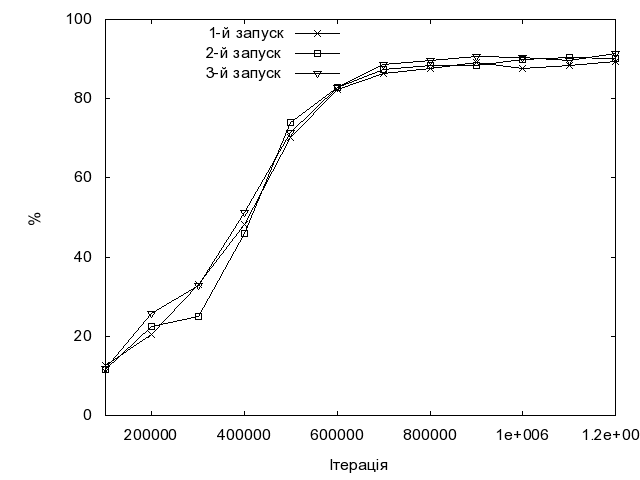
\includegraphics[width=0.3\textwidth]{7-4-linear-spikes_r}}\,
  \subfloat[Зіткнення]{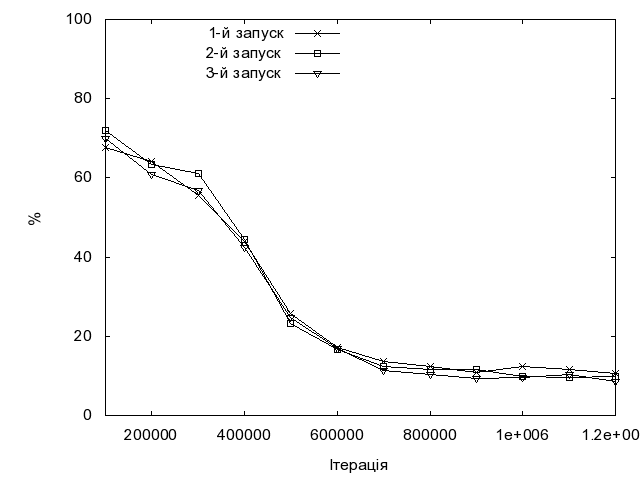
\includegraphics[width=0.3\textwidth]{7-4-linear-spikes_c}}\,
  \subfloat[Таймаут]{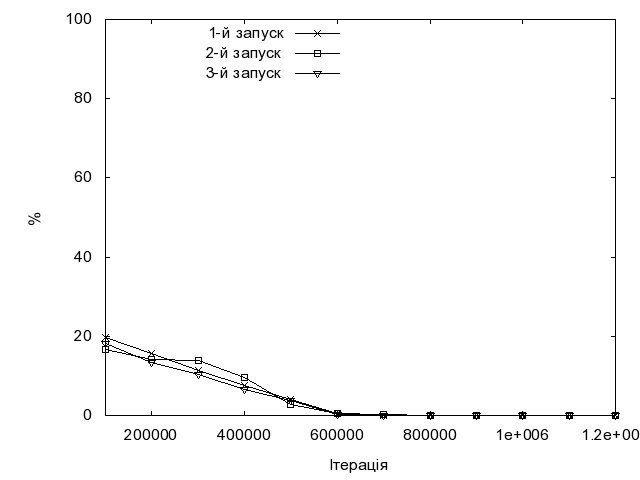
\includegraphics[width=0.3\textwidth]{7-4-linear-spikes_t}}
  \caption{Нейромережа: 7-4-1, eta-linear, eps-spikes}
  \label{fig:7-4-linear-spikes}
\end{figure}

Отримавши такі результати, ми спробували перевірити наскільки впливає на успішність агента розмір нейромережі. Вибравши для тестів найбільш стабільну (згідно попередніх тестів) комбінацію функцій: \textit{eta-spikes} та \textit{eps-spikes}, ми запустили тести для нейромереж наступних конфігурацій: 3-2-1, 5-3-1 та 7-4-1. Отримані результати (рис.~\ref{fig:spikes-spikes-3}, \ref{fig:spikes-spikes-5}, \ref{fig:spikes-spikes-7}) наводять на цікавий висновок: для успішного навчання агента в поставленій задачі зовсім не потрібна велика нейромережа, з поставленим завданням справляється як нейромережа структури 10-6-1, так і невелика структури 3-2-1.

\begin{figure}[h]
  \centering
  \subfloat[Успіх]{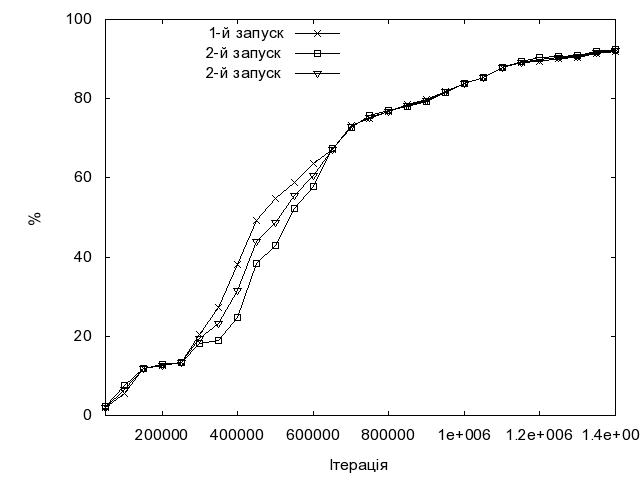
\includegraphics[width=0.3\textwidth]{3-2-s-s_s3_r}}\,
  \subfloat[Зіткнення]{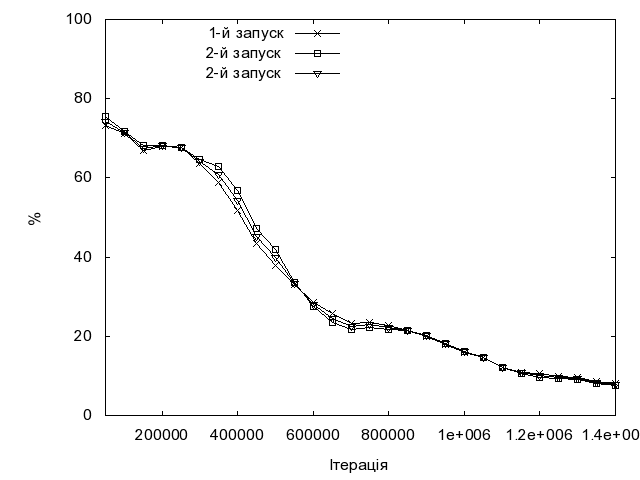
\includegraphics[width=0.3\textwidth]{3-2-s-s_s3_c}}\,
  \subfloat[Таймаут]{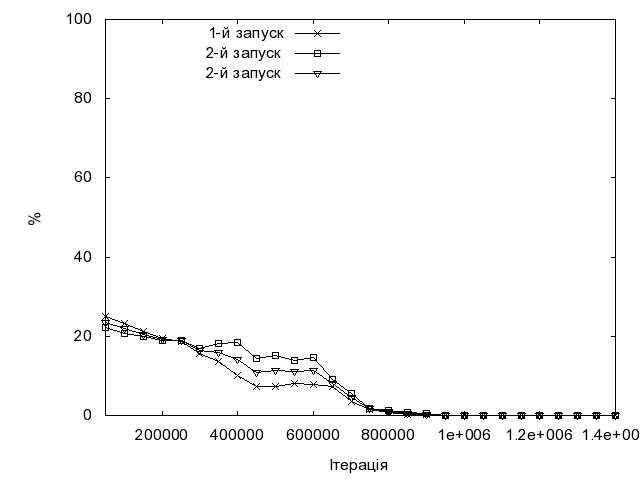
\includegraphics[width=0.3\textwidth]{3-2-s-s_s3_t}}
  \caption{Нейромережа: 3-2-1}
  \label{fig:spikes-spikes-3}
\end{figure}

\begin{figure}[h]
  \centering
  \subfloat[Успіх]{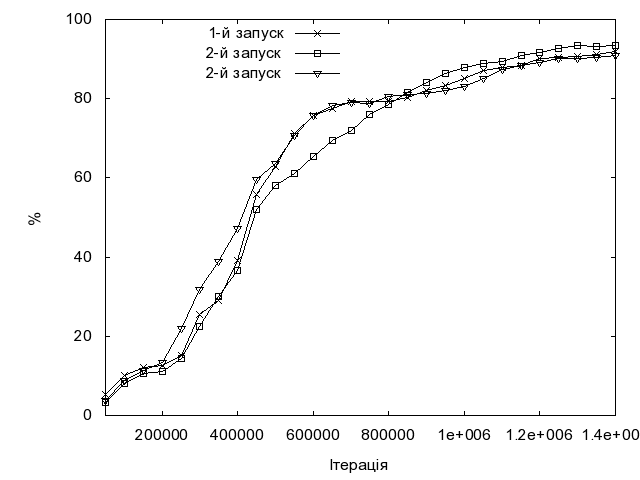
\includegraphics[width=0.3\textwidth]{5-3-s-s_s3_r}}\,
  \subfloat[Зіткнення]{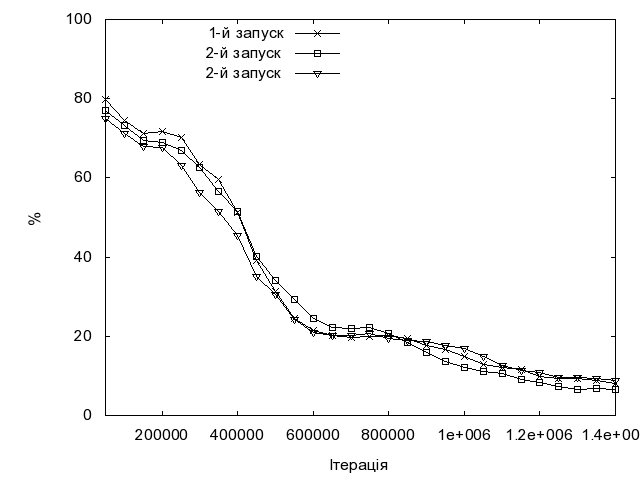
\includegraphics[width=0.3\textwidth]{5-3-s-s_s3_c}}\,
  \subfloat[Таймаут]{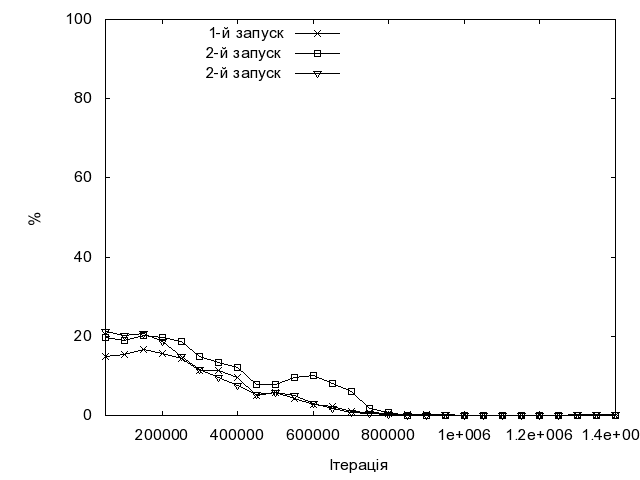
\includegraphics[width=0.3\textwidth]{5-3-s-s_s3_t}}
  \caption{Нейромережа: 5-3-1}
  \label{fig:spikes-spikes-5}
\end{figure}

\begin{figure}[h]
  \centering
  \subfloat[Успіх]{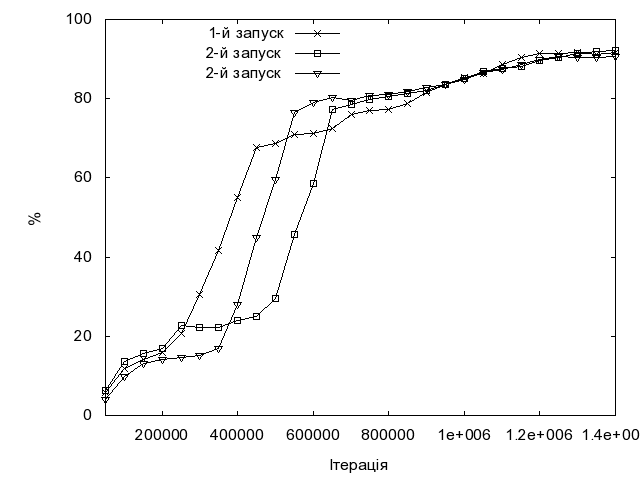
\includegraphics[width=0.3\textwidth]{7-4-s-s_s3_r}}\,
  \subfloat[Зіткнення]{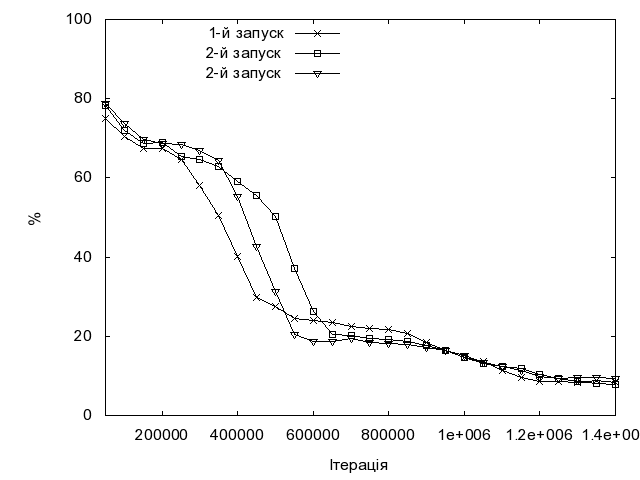
\includegraphics[width=0.3\textwidth]{7-4-s-s_s3_c}}\,
  \subfloat[Таймаут]{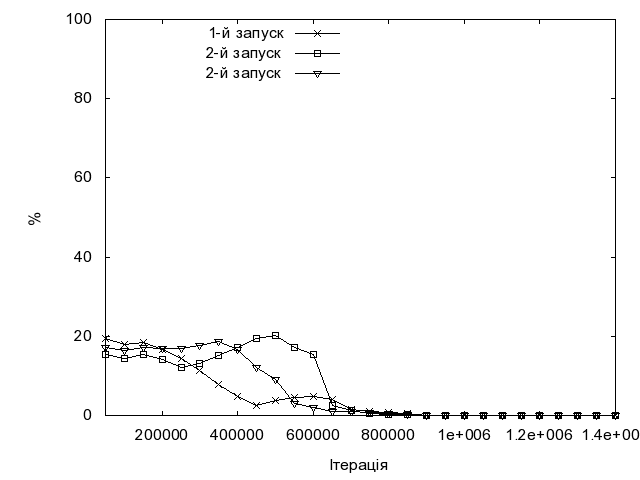
\includegraphics[width=0.3\textwidth]{7-4-s-s_s3_t}}
  \caption{Нейромережа: 7-4-1}
  \label{fig:spikes-spikes-7}
\end{figure}

\clearpage

\section{Висновки}

Використовуючи парадигму навчання з підсиленням, ми створили контролер навігації робота, який базуючись на обмеженій інформації про навколишній світ, забезпечує добирання робота до цілі, уникаючи зіткнення з перешкодами. Як показали практичні експерименти, розроблений контролер є досить ефективним і забезпечує успішне добирання до цілі в абсолютній більшості випадків (в середньому $87\%-92\%$).

Якщо порівнювати використаний підхід, з попереднім підходом на базі системи експертних правил, використаним нами раніше, можна відзначити, що навчання з підсиленням забезпечує значно більшу гнучкість, даючи можливість змінювати структуру стану системи, без жодних інших ускладнень. У випадку з системою експертних правил, така зміна одразу приводить до труднощів, оскільки потрібно розробляти абсолютно нову систему правил, що є надзвичайно трудомістким та складним процесом. На жаль, досить важко в кількісному відношенні порівняти два зазначених підходи, оскільки, по-перше, завдання агента в цих двох задачах були дещо різні: просто оминання перешкод в випадку з системою правил та добирання до цілі з оминанням перешкод у випадку з навчанням з підсиленням. По-друге, фізика моделей автомобіля та робота суттєво відрізняється, що унеможливлює об'єктивне порівняння. Проте, суб'єктивно, поведінка самостійно навченого робота виглядає значно раціональнішою, природнішою та більш адекватною, порівняно з поведінкою автомобіля у схожих ситуаціях (наприклад, при під'їзді до близько розташованої перешкоди).

Варто зазначити, що в обидвох підходах є як позитивні, так і негативні сторони. Для підходу на базі експертних правил характерним є швидкий процес навчання, проте сама розробка правил досить громіздка. Для навчання з підсиленням навпаки: немає затрат часу та сил на розробку системи правил, оскільки мобільний агент сам розробляє свої внутрішні правила, проте процес навчання триває досить довго. Для прикладу, здійснення 2 мільйонів навчальних кроків на середньостатистичному комп'ютері триває більше однієї години. Неоднозначним для навчання з підсиленням є його залежність від евристичних параметрів: зміна параметру $\varepsilon$ у $\varepsilon$-жадібній стратегії вибору дій з константного значення $0.1$ на лінійно-спадну послідовність від $0.2$ до $0.01$ призвело до покращення результатів на $5\%-10\%$. Сильну залежність ефективності та стабільності навчання з підсиленням від вибору $\varepsilon$-функції стратегії вибору дій та $\eta$-функції кроку навчання нейромережі добре видно з експериментів описаних вище.

Можливо, саме така залежність навчання з підсиленням від евристичних параметрів є поясненням того, що розроблена нами система контролю за своїми показниками поступається схожій системі, розробленій G.A.~Rummery~(\cite{Rummery1995}), для якої характерними були показники рівня успішності робота в межах $96\%-99\%$. Можливо, більш якісним підбором різноманітних евристичних параметрів навчання можна було б досягти ефективнішої поведінки агента.

Тим не менше, зручність та легкість внесення змін у структуру середовища, його стану чи фізики моделі без зміни навчального процесу, а також хороші показники ефективності навченого агента "--- безсумнівні переваги навчання з підсиленням. У випадку з проблемою навігації, незначна зміна сприймання роботом навколишнього середовища таким чином, щоб поле зору мінімально захоплювало територію зліва та справа від нього, без будь-яких інших вдосконалень дає покращення результатів на $15\%-17\%$. 

Особливої уваги заслуговує використання штучної нейромережі у якості апроксиматора функції. Хороші властивості апроксимації та узагальнення нейромережі "--- основна складова успішного застосування навчання з підсиленням для складних проблем з неперервним простором станів, як у випадку з навігацією агента. Нейромережа показала себе чудовим інструментом, який доповнює парадигму навчання з підсиленням. Цікаво, що, незважаючи на те, що в літературі досі не було дано будь-яких теоретичних доведень та умов збіжності алгоритмів навчання з підсиленням при використанні нелінійних апроксиматорів функцій, вкотре було показано практичну застосовність штучних нейромереж в якості функцій корисності для алгоритмів навчання з підсилення у складних задач контролю. 

Щоправда, нейромережа вносить додатковий рівень складності у розроблені алгоритми, вимагаючи обережного та точного підбору параметрів навчання самої нейромережі, а також вибору оптимальної структури, кількості нейронів та їх активаційних функцій.

Загалом, індуктивні методи навчання є дуже перспективним напрямком роботи, оскільки дають можливість створювати ефективні контролери для задач, з якими дедуктивні методи не справляються через складність та неоднозначність поставленого завдання.

\addcontentsline{toc}{section}{Література}
\begin{thebibliography}{99}
\bibitem{Rummery1995}{Rummery, G. A. 1995. Problem Solving with Reinforcement Learning. Ph.D. thesis. Cambridge University Engineering Department.}
\bibitem{SuttonBarto2002}{Sutton, R. S., Barto, A. G. 2002. Reinforcement Learning: An Introduction. A Bradford Book, The MIT Press, Cambridge, Massachusetts, London, England.}
\bibitem{Coulom2002}{Coulom, R. 2002. Reinforcement Learning Using Neural Networks, with Applications to Motor Control. Ph.D. thesis. Institut National Polytechnique de Grenoble.}
\bibitem{Kaelbling1996}{Kaelbling L., Littman M., Moore A. 1996. Reinforcement Learning: A Survey. Journal of Artificial Intelligence Research 4, 1996, 237-285}
\bibitem{Kun03}{Phіlіppe Kunzle. Vehіcle Control wіth Neural Networks "--- http://www.gamedev.net/reference/artіcles/artіcle1988.asp}
\end{thebibliography}

\end{document}
